\chapter{Background}
\label{chap:background}

\begin{fquote}[G-Man][Half-Life 2]
  The right man in the wrong place can make all the difference in the world.
\end{fquote}

In this chapter we review some definitions and notations used in this thesis. We limit ourselves to the basic notations used during the work. However, the bibliography of each subject will be referenced for further details about the topic.

%\todo{Text about background intro}

%%% This is an example first chapter.  You should put chapter/appendix that you
%% write into a separate file, and add a line \include{yourfilename} to
%% main.tex, where `yourfilename.tex' is the name of the chapter/appendix file.
%% You can process specific files by typing their names in at the
%% \files=
%% prompt when you run the file main.tex through LaTeX.
\section{Graphs and intersections}
\label{sec:graphs}


\subsection{Graphs}

A graph $G$ is defined as $G = (V,E)$, where $V$ is the set of vertices and $E$ the set of
edges, where $E \subseteq \binom{V}{2}$. The vertices $v,w \in V$ such that $e = vw \in E$
links are called the \textit{endpoints} of $e$.

\begin{defn}
  An embedding of a graph $G$ into a surface $\Sigma$ is a mapping of $G$ in
  $\Sigma$ where the vertices correspond to distinct points and the edges
  correspond to simple arcs connecting the images of their endpoints.
  \cite{goyalGraphEmbeddingTechniques2017}.
\end{defn}

A graph $G$ is planar if there is an embedding of this graph that does not have
any crossing between the edges.

\begin{defn}
  Let $G = (V,E)$ and $S \subset V$, an induced subgraph is a graph $H$ of $G$ whose
  vertex set is $S$ and its edge set $F = \{vw : v,w \in S, vw \in E\}$.
\end{defn}

\begin{defn}
  Let $G = (V,E)$ its complement graph $\overline{G}$ is the graph such that its edge set
  is defined as: $\{vw: v,w\in V, vw\notin E\}$.
\end{defn}

\begin{defn}
  $H$ is called a \textit{minor} of $G$ if $H$ can be constructed by deleting edges and vertices,
  or contracting edges.
\end{defn}

\begin{theorem}[Kuratowski]
  A graph $G$ is planar if and only if it does not contain $K_5$ or $K_{3,3}$ as a minor or
  a induced subgraph.
\end{theorem}

\begin{defn}
  A path $P_n$ in a graph $G$ is a sequence of vertices $v_1v_2v_3\dots v_n$ such
  that $v_iv_{i+1} \in E$.
\end{defn}

\begin{defn}
  A cycle $C_n$ in a graph $G = (V,E)$ is a path $v_1\dots v_n$ such that $v_1 = v_n$.
\end{defn}

\begin{defn}
  A chord of a cycle $C_n$ is an edge that connects two non consecutive vertices
  of $C_n$.
\end{defn}

\begin{defn}
  A graph $G = (V,E)$ is complete if every pair of distinct $v_1,v_2 \in V$ are
  adjacent. This is denoted $K_n$ with $n$ the size of the graph. If $G$ is an
  induced graph of $H$ then $G$ is a clique of $H$.
\end{defn}

\begin{defn}
  A graph $G$ is bipartite if there exist two disjoint subsets $A,B \subset V$ such
  that $A\cup B = V$ and each edge $e\in E$ has an endpoint on $A$ and the
  another on $B$.
\end{defn}

\begin{defn}
  A bipartite graph $G$ with bipartitions $A$ and $B$ is complete bipartite if
  every pair of vertices $v\in A, w\in B$ are adjacent. It is denoted as $K_{n,m}$,
  being $n$ and $m$ the size of each bipartition.
\end{defn}

\begin{defn}
  An induced forbidden subgraph of a graph class $X$ is a graph such that if it is the induced
  subgraph of a graph $G$, we know that $G \notin X$.
\end{defn}

The coloration of a graph is a color assignment to each vertex such that the color
of the two endpoints of every edge of the graph is different.

\begin{defn}
  The chromatic number of a graph $\chi(G)$ is the smallest number of colors needed to
  have an acceptable coloration of $G$.
\end{defn}

\begin{defn}
  The clique number of a graph $\omega(G)$ is the size of the biggest clique of $G$. We
  can observe that for every graph: $\chi(G) \geq \omega(G)$.
\end{defn}

\begin{defn}
  A perfect graph is a graph that respects this condition for every induced subgraph:
  $$ \omega(G) = \chi(G)$$
\end{defn}

\begin{theorem}[Lovasz]
  $G$ is perfect if and only if $\overline{G}$ is perfect.
\end{theorem}

\subsection{Intersection graphs}

\begin{defn}
The \textit{intersection graph} of a collection $\zeta$ of objects is the graph
$(\zeta,E)$ such that $c_1c_2\in E \Leftrightarrow c_1 \cap c_2 \neq \varnothing$.
\end{defn}


\begin{defn}
  A partial order is a binary relation $\leq$ over a set $A$ satisfying these axioms:
  \begin{itemize}
    \item $a \leq a$ (reflexivity).
    \item if $a \leq b$ and $b \leq a$ then $a = b$ (antisymmetry).
    \item if $a \leq b$ and $b \leq c$ then $a \leq c$ (transitivity).
  \end{itemize}
\end{defn}

\begin{defn}
   A partially ordered set or poset  $(S,\leq)$ where $S$ a set and $\leq$ a partial
   order on $S$.
\end{defn}

\begin{defn}
  A graph $G = (V,E)$ is a comparibility graph if there exists a partial order
  $\leq$ such that $vw \in E \Leftrightarrow v \leq w$ or $w \leq v$.
  Equivalently, $G$ is a comparability graph if it is the comparability graph of
  a poset. For example, the Hasse diagram (figure \ref{fig:hasse}) is a
  comparability graph where the relation is inclusion.
\end{defn}

\begin{figure}
\centering

\begin{scaletikzpicturetowidth}{\textwidth}
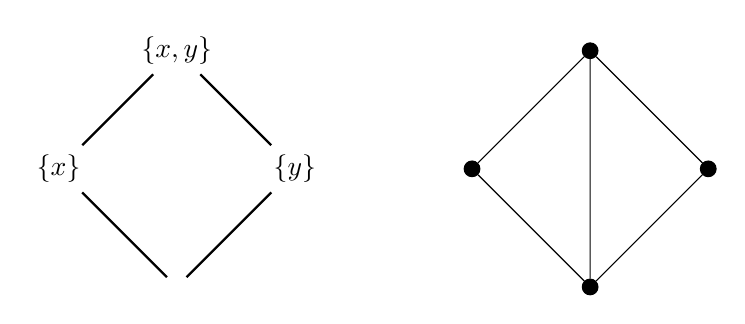
\begin{tikzpicture}[scale=1.5]

  % poset
  \draw (-1cm,0cm) node (v2) {$\{x\}$};
  \draw (1cm,0cm)  node (v3) { $\{y\}$ };
  \draw (0cm,-1cm) node (v4) {$\varnothing$};
  \draw (0cm,1cm)  node (v1) {$\{x,y\}$};

  \draw[thick]  (v1) edge (v2);
  \draw[thick]  (v3) edge (v1);
  \draw[thick]  (v3) edge (v4);
  \draw[thick]  (v2) edge (v4);

  % graph
  \node[draw,circle,inner sep=2pt,fill,label distance=1cm] (v1g) at (3.5,1) {};
  \node[draw,circle,inner sep=2pt,fill,label distance=1cm] (v2g) at (3.5,-1) {};
  \node[draw,circle,inner sep=2pt,fill,label distance=1cm] (v3g) at (4.5,0) {};
  \node[draw,circle,inner sep=2pt,fill,label distance=1cm] (v4g) at (2.5,0) {};
  \draw  (v1g) edge (v2g);
  \draw  (v1g) edge (v4g);
  \draw  (v4g) edge (v2g);
  \draw  (v1g) edge (v3g);
  \draw  (v3g) edge (v2g);

\end{tikzpicture}
\end{scaletikzpicturetowidth}

\caption{On the left, Hasse diagram of a poset of the power set of 2 elements ordered by inclusion.
On the right, the comparability graph of this poset.}
\label{fig:hasse}
\end{figure}

\subsubsection{Interval graphs}

An interval graph is a graph $G$ that is the intersection graph of a collection
of closed intervals in $\mathbb{R}$. If the length of each interval is unitary,
then $G$ is a unit interval graph (UIG).

\begin{theorem}
  $G$ is an interval graph if and only if every simple cycle of four or more
  points has a chord. \cite{FISHBURN1985135}
\end{theorem}

\begin{theorem}
  An interval graph is a unit interval graph if and only if it has no induced subgraph $K_{1,3}$ \cite{roberts1968representations}.
\end{theorem}

Another interesting class of interval graphs are mixed unit interval graphs, where each
interval can be closed, open, open-closed or closed-open. In this paper we will
denote those four classes like this:

$$\mathcal{I}^{++} = \{[x,y] : x,y \in \mathbb{R}, x\leq y\}$$
$$\mathcal{I}^{--} = \{(x,y) : x,y \in \mathbb{R}, x\leq y\}$$
$$\mathcal{I}^{+-} = \{[x,y) : x,y \in \mathbb{R}, x\leq y\}$$
$$\mathcal{I}^{-+} = \{(x,y] : x,y \in \mathbb{R}, x\leq y\}$$

$\mathcal{I}$ will be replaced by $\mathcal{U}$ when we are talking about unit
mixed interval graphs and their class is denoted MUIG.

\begin{theorem}
  The classes of the graphs $\mathcal{U}^{--}$, $\mathcal{U}^{++}$,
  $\mathcal{U}^{-+}$, $\mathcal{U}^{+-}$, and  $\mathcal{U}^{-+} \cup
  \mathcal{U}^{+-}$ are the same (equivalent for $\mathcal{I}$). \cite{DOURADO20123357}
\end{theorem}



\begin{figure}
\centering


\begin{scaletikzpicturetowidth}{\textwidth}
\begin{tikzpicture}[scale=1.5]

  \draw[{(-)}] (-1,-0.5) -- (0,-0.5);
  \draw[color=black] (-0.4845,-0.8507) node {$v_4$};
  \draw[{[-}] (0,-1.5) -- (1,-1.5);
  \draw[color=black] (0.5023,-1.3568) node {$v_3$};
  \draw[{-]}] (-2,-1.5) -- (-1,-1.5);
  \draw[color=black] (-0.4899,-0.3468) node {$v_2$};
  \draw[{[-]}] (-1,-1) -- (0,-1);
  \draw[color=black] (-1.4962,-1.3536) node {$v_1$};

  \node[draw,circle,inner sep=2pt,fill,label distance=1cm] (v1) at (-4,-0.25) {};
  \draw[color=black] (-4,0) node {$v_4$};
  \node[draw,circle,inner sep=2pt,fill,label distance=1cm] (v3) at (-4,-1.25) {};
  \draw[color=black] (-4,-1.5) node {$v_2$};
  \node[draw,circle,inner sep=2pt,fill,label distance=1cm] (v2) at (-5,-1.25) {};
  \draw[color=black] (-3,-1.5) node {$v_3$};
  \node[draw,circle,inner sep=2pt,fill,label distance=1cm] (v4) at (-3,-1.25) {};
  \draw[color=black] (-5,-1.5) node {$v_1$};
  \draw  (v1) edge (v2);
  \draw  (v1) edge (v3);
  \draw  (v1) edge (v4);

\end{tikzpicture}
\end{scaletikzpicturetowidth}

\caption{Representation of $K_{1,3}$ as a MUIG.}
\label{fig:muigK13}
\end{figure}

Unlike for UIG class, $K_{1,3}$ is a MUIG as seen in figure \ref{fig:muigK13}. Some
characterizations have been already found for these classes of graphs \cite{shuchatUnitMixedInterval2014a}
\cite{joosCharacterizationMixedUnit2013}.

\todo[inline]{Exploit these characterizations!! $\to$ explain them and use them to characterize UUIG.}

\subsubsection{Disks}

A disk graph $G$ is a graph that is an intersection graph of disks on the plane, when the size
of the disk is unitary, we talk about unit disk graphs. This class of graphs
is important for this thesis, as thin strip graphs are a sub-class of
unit disk graphs.

We will refer to the unit disk graph class as UDG and an example of a realization
can be found in the figure \ref{fig:udg}.

\paragraph{Induced forbidden subgraphs} The characterization of this class with respect to
its induced forbidden subgraphs has been studied \cite{atminasForbiddenInducedSubgraphs2016}.

\begin{theorem}[Atminas-Zamaraev]
  For every integer $k > 1$, $\overline{K_2 + C_{2k+1}}$ is a minimal induced subgraph.
\end{theorem}

\begin{theorem}[Atminas-Zamaraev]
  For every integer $k > 4$, $\overline{C_{2k}}$ is a minimal induced subgraph.
\end{theorem}

\begin{figure}
\centering

\begin{scaletikzpicturetowidth}{\textwidth}
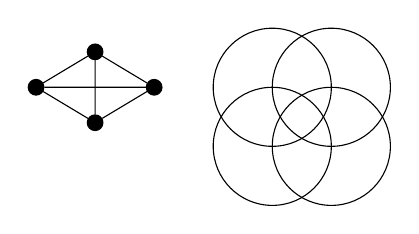
\begin{tikzpicture}[scale=1.5]

  \draw (-0.5,2.5) circle [radius=0.5];
  \draw (0,2.5) circle [radius=0.5];
  \draw (-0.5,2) circle [radius=0.5];
  \draw (0,2) circle [radius=0.5];


  \node[draw,circle,inner sep=2pt,fill,label distance=1cm] (v1) at (-2.5,2.5) {};

  \node[draw,circle,inner sep=2pt,fill,label distance=1cm] (v2) at (-2,2.2) {};
  \node[draw,circle,inner sep=2pt,fill,label distance=1cm] (v3) at (-2,2.8) {};
  \node[draw,circle,inner sep=2pt,fill,label distance=1cm] (v4) at (-1.5,2.5) {};

  \draw  (v3) edge (v2);
  \draw  (v4) edge (v1);
  \draw  (v3) edge (v1);
  \draw  (v4) edge (v2);
  \draw  (v3) edge (v4);
  \draw  (v1) edge (v2);

\end{tikzpicture}
\end{scaletikzpicturetowidth}

\caption{Realization of a UDG (Unit Disk Graph).}
\label{fig:udg}
\end{figure}

%%% This is an example first chapter.  You should put chapter/appendix that you
%% write into a separate file, and add a line \include{yourfilename} to
%% main.tex, where `yourfilename.tex' is the name of the chapter/appendix file.
%% You can process specific files by typing their names in at the
%% \files=
%% prompt when you run the file main.tex through LaTeX.
\section{Complexity}
\label{sec:complex}

Complexity theory has the objective to establish lower bounds on how efficient
an algorithm can be for a given problem \cite{sipserIntroductionTheoryComputation2006}. This approach let us
have a reference point to establish the difficulty of a problem.


\begin{defn}
Let $\Sigma$ be a finite alphabet, $\Sigma^*$ every word derived from $\Sigma$, $L \subseteq \Sigma^*$ is a decision problem.
\end{defn}

\begin{defn}
  A decider for a decision problem $A$ is an deterministic algorithm $V$ where
    $$A = \{w | V \textit{accepts } w\}$$
  $A$ is polynomially decidable if it has a polynomial time decider \cite{sipserIntroductionTheoryComputation2006}.
\end{defn}

\begin{defn}
A verifier for a decision problem $A$ is an deterministic algorithm $V$ where
  $$A = \{w | V \textit{accepts } \langle w,c\rangle \textit{ for some string } c\}$$
$A$ is polynomially verifiable if it has a polynomial time verifier \cite{sipserIntroductionTheoryComputation2006}.
\end{defn}

\subsection{P vs NP}

\begin{defn}
A problem $L \in \mathcal{P}$ if $L$ is polynomially decidable.
\end{defn}

\begin{defn}
A problem $L \in \mathcal{NP}$ if $L$ is polynomially verifiable. Thus, $\mathcal{P} \subseteq \mathcal{NP}$.
\end{defn}

To prove a bound of complexity on an unknown problem $L$ we have to find another
problem with already known complexity and find equivalences between those two. This
can be achieved through \textit{reductions}.

\begin{defn}
  A reduction of a problem $L$ to a problem $M$ is a mapping of an instance of $L$ ($I_L$)
  to an isntance of $M$ ($I_M$) such that $I_L$ is true for the problem $L$ if and
  only if $I_M$ is true for the problem $M$. This is noted $L \leq M$ and $L \leq_P M$
  if the reduction is done in polynomial time.
\end{defn}

With this concept we can define new complexity classes. $\mathcal{NP}$-hard is
the set of problems so that we can reduce every $\mathcal{NP}$ problem to. The set
of problems that are both $\mathcal{NP}$-hard and $\mathcal{NP}$ are called $\mathcal{NP}$-complete.
This is generalized to every complexity class ($\mathcal{P}$, $\exists \mathbb{R}$, RP, etc...)

\paragraph{Satisfiability problem} The satisfiability problem (SAT) is to decide the satisfiability
of a CNF formula $\phi$. A CNF formula is a boolean formula that is a conjunction of multiple
clauses $c_k$. A clause is a disjunction of multiple literals. A literal may be a variable
or a negation of a variable.

\begin{theorem}[Cook-Levin]
  SAT is $\mathcal{NP}$-complete.
\end{theorem}

\paragraph{Clique problem} The clique problem is to find a maximum clique of a graph
$G$.

\begin{theorem}
  CLIQUE is $\mathcal{NP}$-complete. \cite{Karp1972}
\end{theorem}

\begin{theorem}
  CLIQUE is QPTAS when applied to disk graphs. \cite{DBLP:journals/corr/abs-1712-05010}
\end{theorem}

\begin{theorem}[Clark-Colbourn]
  CLIQUE is $\mathcal{P}$ when applied to unit disk graphs. \cite{CLARK1990165}
\end{theorem}

\subsection{$\exists \mathbb{R}$ complexity class}

$\exists \mathbb{R}$ is the class that describes the problems that can be reduced to
\textit{the existential theory of the reals}\cite{ExistentialTheoryReals2006a}. The
existential theory of the reals is the problem of deciding if a sentence of this form
is true:

$$(\exists X_1 \dots \exists X_n): F(\exists X_1, \dots,\exists X_n)$$\\

where $F$ is a quantifier-free formula in the reals. In other words, it is a
conjuntion of clauses where each clause is a real polynomial inequality where
each variable $X_k$ is a real number. We can see that ETR is NP-hard because
SAT can be reduced to it.


\begin{proof}
  Let's take an instance of SAT $\phi_{SAT}$ with clauses $c_k$ and variables
  $x_k$, we can construct an instance of ETR $\phi_{ETR}$ where we can
  construct variables in the domain $\{0,1\}$ with this equality, so for each
  variable $X_k$:
  $$X_k - X_k^2 = 0$$

  Each literal of each clause will be positive or negative depending if the literal is cancelled in $\phi_{SAT}$:

  $$x_k \to l = X_k$$
  $$\neg x_k \to l = (1-X_k)$$

  Then for each clause we can have a polynomial for which the sum of the values of every
  literal in the clause must be greater than one, so that at least one literal is true:

  $$\sum_{l\in c_k} l \geq 1$$

  With this proof, it is easy to see that $\phi_{ETR}$ is valid if and only if $\phi_{SAT}$ is also valid.  \qed\\

\end{proof}

This result can show us that $P \subseteq NP \subseteq \exists \mathbb{R}$.

\subsubsection{Problems in $\exists \mathbb{R}$}

In this section we will describe some problems that are $\exists
\mathbb{R}$-complete and will give an overview of the proof.

\paragraph{The art gallery problem} Given a simple polygon $P$ (without
crossings between every side), we introduce \textit{guards}. A guard
$g$ is a point such that every point of the polygon is watched by a guard.
A point $p$ is watched by a point $q$ if the segment $pq$ is contained
in $P$. The subset $G$, being $G$ the set of guards and $G \subseteq
P$, is optimum if it has the minimal cardinality covering the whole
polygon.

The art gallery problem is to decide, given a polygon $P$ and a number of
guards $k$, whether there exists a configuration of $k$ guards in $G$
guarding the whole polygon. The art gallery problem is $\exists
\mathbb{R}$-complete \cite{abrahamsenArtGalleryProblem2017}.

\paragraph{Proof idea} First of all, we can see that the art gallery problem
is in $\exists \mathbb{R}$ if we reduce this problem to ETR. If we have an
instance $(P,k)$ of the art gallery problem we can have a formula
\cite{EFRAT2006238} like this:

$$\phi = \{\exists x_1y_1,\dots x_ky_k \forall p_xp_y :
\text{INSIDE-POLYGON}(p_x,p_y) \to \bigvee_{1 \leq i \leq k}
\text{SEES}(x_i,y_i,p_x,p_y)\}$$

Where INSIDE-POLYGON returns $1$ if $(p_x,p_y) \in P$ and SEES returns $1$ if
the segment $(x,y)(p_x,p_y) \in P$. $\phi$ is not a ETR formula, so we would like
to construct a quantifier-free formula with the idea of $\phi$. To achieve this,
the main idea is to have a small set of points $Q \subseteq P$ such that if these
points are watched, the whole polygon is watched. This subset $Q$ is called
the \textit{witness set}. The only thing is now to create a polynomial for each
point that ensures that the point is watched by a guard.

To finish the proof we have to prove that the art gallery problem is $\exists
\mathbb{R}$-hard. For this part an $\exists \mathbb{R}$-complete
problem has been deducted from ETR. For the problem ETR-INV we have a set of
variables $\{x_1,\dots,x_n\}$ and a set of equations of this form:

$$x = 1,\ \ x + y = z,\ \ x \cdot y = 1 $$

and the problem decides if it exists a solution to this set of equations such
that the value of each variable is real in $[\frac{1}{2},2]$.

A reduction of ETR-INV is found to the art gallery problem by constructing
a polygon $P$ and finding a number $g$ for that polygon such that the instance
of ETR-INT is true if and only if $P$ is covered by at most $g$ guards.

\paragraph{Stretchability} A pseudoline is a simple closed curve in the plane.
The stretchability problem is to decide if given a pseudoline arrangement,
it is equivalent to an arrangement of straight lines.

\paragraph{Proof idea} ETR can be reduced to STRETCHABILITY due to Mnev's
universality theorem. \cite{10.1007/978-3-642-11805-0_32}

\paragraph{Unit disk graph recognition} The unit disk graph recognition is
the problem that decides if a graph $G$ is a unit disk graph. Unit disk graph
recognition is $\exists \mathbb{R}$-complete. \cite{Schaefer2013}

\paragraph{Proof idea} UDG recognition is a corollary of deciding whether a graph
with a given length is realizable. This problem is $\exists \mathbb{R}$-complete.

The reduction is done from STRETCHABILITY \cite{Schaefer2013}. The reduction is
done by adding a vertex to $V$ for each pseudoline intersection. For each three
consecutive points $u_1, u_2, u_3$ along a pseudoline a widget will be added that will
be only realizable if and only if the pseudoline can be stretched with the same
arrangement.

%%% This is an example first chapter.  You should put chapter/appendix that you
%% write into a separate file, and add a line \include{yourfilename} to
%% main.tex, where `yourfilename.tex' is the name of the chapter/appendix file.
%% You can process specific files by typing their names in at the
%% \files=
%% prompt when you run the file main.tex through LaTeX.
\section{Geometry}
\label{sec:geom}

The intersection of convex objects is a matter well studied for multiple
subjects. In our case, it is interesting to know some properties about
the intersection of disks, those ones being convex objects.

A set $S$ is convex if:
$$\forall p,q \in S\  \forall \lambda \in [0,1]: (1-\lambda)p + \lambda q \in S$$

\subsection{Stabbing}
A \textit{stabbing} is a point that traverses a set of intersecting objects. A lot of
research has been done \cite{schlipf2013stabbing} on the minimal amount of stabbings to
cover every object in a set. Stabbings can also be done with more complex structures
than points, in that case we are talking about \textit{coverings}.

\begin{theorem}[Helly]
  Given a set $Q$ of objects in $\mathbb{R}^d$, if for each subset of $Q$ of
  size $d+1$ their intersection is non empty, then $\bigcap_{q \in Q} \neq
  \varnothing$. \cite{Helly1923175}
\end{theorem}

\begin{theorem}
  The problem that for a set of $n$ disks whether there exists a regular n-gon
  whose vertices stab every disk of the set can be decided in $O(n^{10.5} / \sqrt{\log(n)})$ \cite{schlipf2013stabbing}
\end{theorem}

\subsection{Coin graphs}

Penny graphs can be defined as disk graphs where the disks can just touch each
other without overlapping. A famous theorem is derived from this class of graphs:
the circle packing theorem.

\begin{theorem}[Circle packing theorem]
  The circle packing theorem states that every simple connected planar graph
  $G$ is a penny graph. \cite{doi:10.1137/0406017}
\end{theorem}

\begin{corollary}
  Planar graphs $\subseteq$ disk graphs \cite{spinradEfficientGraphRepresentations2012}.
\end{corollary}

\begin{figure}
\centering
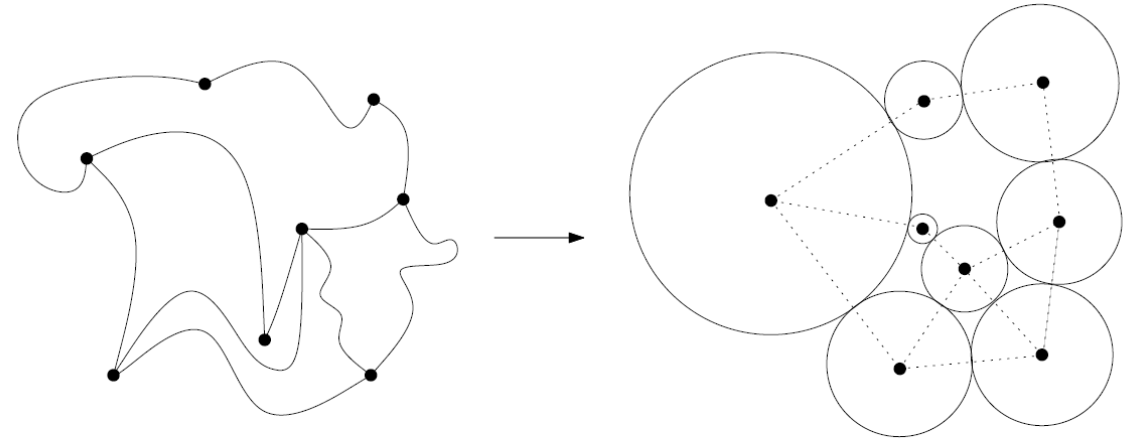
\includegraphics[width=1.0\textwidth]{res/circle_packing}
\caption{Circle packing of a planar graph. \cite{nachmiasPlanarMapsRandom2016}}
\label{fig:circle}
\end{figure}


\section{Graph theory}

A \emph{graph} is defined as a tuple $G = (V,E)$ where $V$ is the set of \emph{vertices} and $E$ is a set of \emph{edges} where $E = \binom{V}{2}$. An \emph{orientation} of a graph $G$ is an assignment of a direction to each edge, we denote the orientation of the edges by $\overrightarrow{E}$. An orientation is \emph{transitive} if $uv \in \overrightarrow{E}$ and $vw in \overrightarrow{E}$, then $uw \in \overrightarrow{E}$. If two vertices are share the same edge $e$ they are called \emph{adjacent} and also the \emph{endpoints} of $e$. A \emph{subgraph} $H = (V', E')$ of a graph $G$ is a graph such that $V' \subseteq V$ and $E' \subseteq E$. An \emph{induced subgraph} of a graph is a subgraph $H$ of a graph $G$ such that for every edge of $G$ is also in $H$ if its two endpoints are in $V'$. A \emph{clique} is a subgraph such that every vertex is adjacent to each other. A graph that is also a clique is called a \emph{complete graph} and it is denoted as $K_n$. A graph is \emph{bipartite} if there exist two disjoint subsets of the vertex set $A \cup B = V$ such that two vertices of the same subset are not adjacent. A \emph{complete bipartite graph} $K_{n,m}$ is a bipartite graph such that $v \in A$ and $w \in B$ implies $vw \in E$ where $n$ and $m$ are the size of each bipartition.

A \emph{path} $P_n = v_1\dots v_{n+1}$ of a graph is a sequence of pairwise distinct $n$ vertices such that two consequent vertices are adjacent. A \emph{cycle} is a path $C_n = v_1\dots v_nv_{n+1}$ such that $v_1=v_{n+1}$. A graph is \emph{connected} if there exists a path between every pair of vertices. A \emph{chord} of a cycle $C_n$ with $n \geqslant 4$ is an edge that connects two non adjacent vertices of the cycle. A graph is \emph{chordal} if there is a chord in every cycle bigger than four.

Some graphs can be characterized with properties. An \emph{isomorphism} between two graphs $G= (V,E)$ and $H = (V', E')$ is a bijection $f : V \to V'$ between the two vertex sets such that $u,v$ are adjacent in $G$ if and only if $f(u), f(v)$ are adjacent in $H$. A graph \emph{property} is a property of the graph that is preserved in all its isomophisms; this will help us to set properties that are based on the abstraction of the graph and not only its drawings. A property is \emph{hereditary} if it is also preserved under all taking subgraphs.

For notation in this thesis, sometimes the class of a certain type of graphs is denoted by its initials (\textit{e.g.} the class of unit interval graphs is denoted by \emph{UIG}) to avoid extreme repetition.

\subsection{Intersection graphs}

\begin{figure}
\centering

\begin{scaletikzpicturetowidth}{\textwidth}
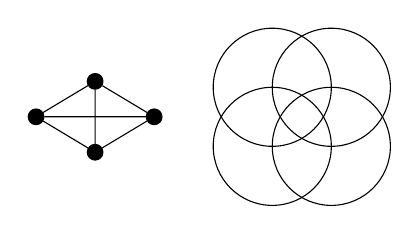
\begin{tikzpicture}[scale=1.5]

  \draw (-0.5,2.5) circle [radius=0.5];
  \draw (0,2.5) circle [radius=0.5];
  \draw (-0.5,2) circle [radius=0.5];
  \draw (0,2) circle [radius=0.5];


  \node[draw,circle,inner sep=2pt,fill,label distance=1cm] (v1) at (-2.5,2.25) {};

  \node[draw,circle,inner sep=2pt,fill,label distance=1cm] (v2) at (-2,1.95) {};
  \node[draw,circle,inner sep=2pt,fill,label distance=1cm] (v3) at (-2,2.55) {};
  \node[draw,circle,inner sep=2pt,fill,label distance=1cm] (v4) at (-1.5,2.25) {};

  \draw  (v3) edge (v2);
  \draw  (v4) edge (v1);
  \draw  (v3) edge (v1);
  \draw  (v4) edge (v2);
  \draw  (v3) edge (v4);
  \draw  (v1) edge (v2);

\end{tikzpicture}
\end{scaletikzpicturetowidth}

\caption{Realization of a UDG (unit disk graph).}
\label{fig:udg}
\end{figure}


An \emph{intersection graph} is a graph $G = (\zeta,E)$ of a collection of objects $\zeta$ is a graph such that $v,w \in \zeta$ and $v \cup w \neq \varnothing$ implies that $vw \in E$. An \emph{interval graph} is an intersection graph of intervals on the plane; when the size of the intervals is equal they are called \emph{unit interval graphs}. A \emph{unit disk graph} is an intersection graph of disks on a plane that have the same diameter - you can find an example in Figure \ref{fig:udg}.\\

For more details about graph theory we recommend

\section{Order and set theory}

The \emph{powerset} $\powerset(S)$ of a set $S$ is the set of subsets of $S$. A \emph{partial order} is a binary relation $\leqslant$ over a set $A$ satisfying three axioms:

\begin{itemize}
  \item if $a \leqslant b$ and $b \leqslant a$ then $a = b$ (\emph{antisymmetry}).
  \item if $a \leqslant b$ and $b \leqslant c$ then $a \leqslant c$ (\emph{transitivity}).
  \item $a \leqslant a$ (\emph{reflexivity}).
\end{itemize}

\begin{figure}
\centering

\begin{scaletikzpicturetowidth}{\textwidth}
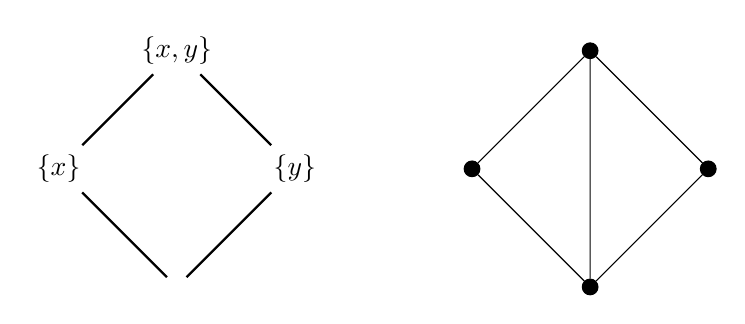
\begin{tikzpicture}[scale=1.5]

  % poset
  \draw (-1cm,0cm) node (v2) {$\{x\}$};
  \draw (1cm,0cm)  node (v3) { $\{y\}$ };
  \draw (0cm,-1cm) node (v4) {$\varnothing$};
  \draw (0cm,1cm)  node (v1) {$\{x,y\}$};

  \draw[thick]  (v1) edge (v2);
  \draw[thick]  (v3) edge (v1);
  \draw[thick]  (v3) edge (v4);
  \draw[thick]  (v2) edge (v4);

  % graph
  \node[draw,circle,inner sep=2pt,fill,label distance=1cm] (v1g) at (3.5,1) {};
  \node[draw,circle,inner sep=2pt,fill,label distance=1cm] (v2g) at (3.5,-1) {};
  \node[draw,circle,inner sep=2pt,fill,label distance=1cm] (v3g) at (4.5,0) {};
  \node[draw,circle,inner sep=2pt,fill,label distance=1cm] (v4g) at (2.5,0) {};
  \draw  (v1g) edge (v2g);
  \draw  (v1g) edge (v4g);
  \draw  (v4g) edge (v2g);
  \draw  (v1g) edge (v3g);
  \draw  (v3g) edge (v2g);

\end{tikzpicture}
\end{scaletikzpicturetowidth}

\caption{On the left, Hasse diagram of a poset of the power set of 2 elements ordered by inclusion.
On the right, the comparability graph of this poset.}
\label{fig:hasse}
\end{figure}

On the other side, a \emph{total order} is a partial order where the reflexivity order is replaced by the \emph{connexity} property -- $a \leq b\ \text{or}\  b \leq a$. A \emph{partially ordered set} (or \emph{poset}) $(S,\leqslant)$ is a set such that the elements of $S$ are partially ordered by the relation $\leqslant$. A good way to represent a poset is the \emph{Hasse diagram} (Figure \ref{fig:hasse}).

\subsection{Comparability graphs}

A \emph{spanning order} $(V,<)$ on a graph $G = (V,E)$ is a total order on $V$ such that for any three vertices $u < v < w$:

  $$uw \in E \to uv \in E\ \text{or}\ vw \in E$$

The class of comparability graphs are built on the ideas of order theory. A graph $G$ is a \emph{comparability graph} if there exists a partial order $\leqslant$ such that $uv \in E \Leftrightarrow v \leqslant w\  \text{or}\  w \leqslant v$. The complement of comparability graphs are called \emph{co-comparability graphs}.


\section{Complexity}

Complexity theory has the objective to establish lower bounds on how efficient an algorithm can be for a given problem. This approach let us have a reference point to establish the difficulty of a problem. A \emph{decision problem} is a problem where we have to decide if a statement is true or false. A \emph{decider} of a decision problem is defined as the deterministic machine that solves this problem. The problem is \emph{polinomially decidable} if it has a polynomial time decider. A \emph{verifier} of a decision problem is a deterministic machine that verifies whether an answer to the decision problem is true or false. Equally, a problem is \emph{polinomially verifiable} if it has a polynomial time verifier. The problem of \emph{recognition} is the problem to decide whether a graph $G$ is in a class of graphs. We denote by $\mathcal{P}$ the class of polinomially decidable problems. On the other hand, $\mathcal{NP}$ denotes the class of polinomially verifiable problems. We can see that $\mathcal{P} \subseteq \mathcal{NP}$.\\

A \emph{reduction} of a problem $L$ to a problem $M$ is a mapping of an instance of $L$ ($I_L$) to an instance of $M$ ($I_M$) such that $I_L$ is true for the problem $L$ if and
only if $I_M$ is true for the problem $M$. This is denoted by $L \leq M$ and $L \leq_P M$ if the reduction is done in polynomial time. We usually prove bounds of complexity for an unknown problem $L$ by reducing it to another problem with an already known complexity. Thus, we can define the class \emph{$\mathcal{NP}$-hard} as the set of problems such that we can reduce every $\mathcal{NP}$ problem to one of them. The set of problems that are both $\mathcal{NP}$ and $\mathcal{NP}$-hard are called \emph{$\mathcal{NP}$-complete}.

\section{Geometry}

We must recall some really basic definitions of geometry. Every geometrical object of this thesis is located in $\mathbb{R}^2$ if it is not otherwise specified. The \emph{distance} between two points as $\text{dist}(a,b)$. An object $S$ is \emph{convex} if for every point $p,q$ the segment between the two points is also contained in $S$. More formally:

$$\forall \lambda \in [0,1]: (1-\lambda)p + \lambda q \in S$$

A \emph{stabbing} is a point that traverses a set of intersecting objects. A lot of research has been done \cite{schlipf2013stabbing} on the minimal amount of stabbings to cover every object in a set. If instead of points we use more complex object, we denote it by a \emph{covering}. The \emph{Helly} theorem says that:

\begin{_theo}[Helly (\cite{Helly1923175}]
  Given a set $S$ of objects in $\mathbb{R}^d$, if for each subset of $S$ of
  size $d+1$ their intersection is non empty, then $\bigcap_{s \in S} \neq
  \varnothing$.
\end{_theo}

We say that a set $S$ satisfies the \emph{Helly property} if every subfamily of $S$ composed of pairwise intersecting objects has also a non-empty intersection. For more details about algorithmic geometry, we recommend the reading of Berg \textit{et al.} \cite{bergComputationalGeometryAlgorithms2008}.
